\pagestyle{fancy}
\fancypagestyle{plain}{}
\cfoot{\Roman{chapter}-\arabic{page}}
\rhead{}
\setcounter{page}{1}
\chapter{HASIL DAN ANALISA PENELITIAN}

\section{Pendahuluan}
Dalam bab ini akan membahas tentang hasil dan analisis dari perangkat lunak analisis sentimen
pada angkutan online menggunakan metode CNN yang telah dibuat pada Bab IV. Hasil data uji ditampilkan
dalam bentuk \emph{confusion matrix} dan tabel laporan hasil klasifikasi pada
Tabel~\ref{tab:format_laporan_hasil_klasifikasi}.


\section{Hasil Penelitian}

\subsection{Konfigurasi Percobaan}
Dalam tahapan ini pengujian dilakukan dengan menggunakan data uji yang telah disiapkan sebanyak 1200
\emph{review} yang terdiri dari 600 label positif dan 600 negatif dan data validasi sebanyak 1200
yang terdiri dari 600 label positif dan 600 label negatif. Pengujian dilakukan sesuai dengan kerangka
kerja penelitian. Hasil penelitian dari pengujian yang dilakukan ditampilkan dalam bentuk berupa
\emph{confusion matrix}, nilai \emph{accuracy}, \emph{precision}, \emph{sensitivity (recall)}, dan
\emph{f-measure (f1-score)}.

Optimasi \emph{parameter} atau \emph{fine-tuning} dilakukan dengan menggunakan data latih dan di
validasi dengan menggunakan data validasi berjumlah 1200 \emph{review} dengan 600 label positif dan 600
label negatif. Pada Tabel~\ref{tab:config_fine_tuning} dapat dilihat parameter dan nilai parameter
yang digunakan untuk mendapatkan parameter model CNN terbaik.

\begin{table}[H]
  \centering
  \caption{Konfigurasi Parameter}
  \label{tab:config_fine_tuning}
  \begin{tabularx}{\columnwidth}{|l|l|}
    \hline
    Parameter            & Nilai                          \\ \hline
    epoch                & 125, 150, 175, 200             \\ \hline
    batch\_size          & 8, 16, 32                      \\ \hline
    activation\_function & softmax, sigmoid               \\ \hline
    loss                 & categorical\_crossentropy, mse \\ \hline
  \end{tabularx}
\end{table} \newpage

\pagestyle{fancy}
\fancypagestyle{plain}{}
\rhead{\Roman{chapter}-\arabic{page}}
\cfoot{}

Berdasarkan konfigurasi parameter pada Tabel~\ref{tab:config_fine_tuning} maka dihasilkan skenario percobaan
yang dapat dilihat pada Tabel~\ref{tab:scenario_fine_tuning}. Semua skenario dari \emph{fine-tuning} dilakukan
dengan menggunakan optimizer = adam, learning\_rate = 0.00001, convolution\_activation = relu,
dan word2vec\_trainable = false.

\begin{longtable}[c]{|l|l|l|l|l|}
  \caption{Skenario Fine-Tuning}
  \label{tab:scenario_fine_tuning}                                                  \\
  \hline
  skenario & epoch & batch\_size & activation\_function & loss                      \\ \hline
  %
  \endhead
  %
  1        & 125   & 8           & softmax              & categorical\_crossentropy \\ \hline
  2        & 150   & 8           & softmax              & categorical\_crossentropy \\ \hline
  3        & 175   & 8           & softmax              & categorical\_crossentropy \\ \hline
  4        & 200   & 8           & softmax              & categorical\_crossentropy \\ \hline
  5        & 125   & 16          & softmax              & categorical\_crossentropy \\ \hline
  6        & 150   & 16          & softmax              & categorical\_crossentropy \\ \hline
  7        & 175   & 16          & softmax              & categorical\_crossentropy \\ \hline
  8        & 200   & 16          & softmax              & categorical\_crossentropy \\ \hline
  9        & 125   & 32          & softmax              & categorical\_crossentropy \\ \hline
  10       & 150   & 32          & softmax              & categorical\_crossentropy \\ \hline
  11       & 175   & 32          & softmax              & categorical\_crossentropy \\ \hline
  12       & 200   & 32          & softmax              & categorical\_crossentropy \\ \hline
  13       & 125   & 8           & sigmoid              & mse                       \\ \hline
  14       & 150   & 8           & sigmoid              & mse                       \\ \hline
  15       & 175   & 8           & sigmoid              & mse                       \\ \hline
  16       & 200   & 8           & sigmoid              & mse                       \\ \hline
  17       & 125   & 16          & sigmoid              & mse                       \\ \hline
  18       & 150   & 16          & sigmoid              & mse                       \\ \hline
  19       & 175   & 16          & sigmoid              & mse                       \\ \hline
  20       & 200   & 16          & sigmoid              & mse                       \\ \hline
  21       & 125   & 32          & sigmoid              & mse                       \\ \hline
  22       & 150   & 32          & sigmoid              & mse                       \\ \hline
  23       & 175   & 32          & sigmoid              & mse                       \\ \hline
  24       & 200   & 32          & sigmoid              & mse                       \\ \hline
\end{longtable}

\subsection{Hasil Percobaan}
Hasil pelatihan dari skenario pada Tabel~\ref{tab:scenario_fine_tuning} dapat dilihat pada
Tabel~\ref{tab:result_training_scenario} dan untuk hasil dari prediksi model yang telah dilatih dengan
menggunakan data uji dapat dilihat pada Tabel~\ref{tab:result_testing_scenario}.

\begin{longtable}[c]{|l|l|l|l|l|}
  \caption{Hasil Skenario Pada Pelatihan}
  \label{tab:result_training_scenario}                                 \\
  \hline
  skenario & train\_accuracy & train\_loss & val\_accuracy & val\_loss \\ \hline
  %
  \endhead
  %
  1        & 99,61\%         & 1,28\%      & 89,50\%       & 29,55\%   \\ \hline
  2        & 99,81\%         & 0,57\%      & 89,25\%       & 29,35\%   \\ \hline
  3        & 99,86\%         & 0,53\%      & 89,75\%       & 28,43\%   \\ \hline
  4        & 99,83\%         & 0,56\%      & 88,58\%       & 29,50\%   \\ \hline
  5        & 98,86\%         & 3,97\%      & 89,33\%       & 29,50\%   \\ \hline
  6        & 99,53\%         & 1,81\%      & 89,42\%       & 28,90\%   \\ \hline
  7        & 99,64\%         & 1,29\%      & 89,50\%       & 29,49\%   \\ \hline
  8        & 99,64\%         & 1,03\%      & 88,67\%       & 29,72\%   \\ \hline
  9        & 96,89\%         & 9,39\%      & 88,83\%       & 29,45\%   \\ \hline
  10       & 98,50\%         & 5,38\%      & 89,08\%       & 29,62\%   \\ \hline
  11       & 98,94\%         & 3,57\%      & 89,25\%       & 29,45\%   \\ \hline
  12       & 99,39\%         & 2,43\%      & 88,33\%       & 30,51\%   \\ \hline
  13       & 99,03\%         & 1,05\%      & 89,17\%       & 8,68\%    \\ \hline
  14       & 99,28\%         & 0,80\%      & 89,25\%       & 8,53\%    \\ \hline
  15       & 99,25\%         & 0,08\%      & 89,33\%       & 8,74\%    \\ \hline
  16       & 99,44\%         & 0,06\%      & 89,17\%       & 8,50\%    \\ \hline
  17       & 97,94\%         & 2,05\%      & 89,00\%       & 8,58\%    \\ \hline
  18       & 98,53\%         & 1,52\%      & 89,17\%       & 8,48\%    \\ \hline
  19       & 99,17\%         & 0,09\%      & 89,50\%       & 8,64\%    \\ \hline
  20       & 99,03\%         & 0,09\%      & 88,92\%       & 8,74\%    \\ \hline
  21       & 96,58\%         & 3,48\%      & 88,75\%       & 8,95\%    \\ \hline
  22       & 97,61\%         & 2,47\%      & 88,92\%       & 8,71\%    \\ \hline
  23       & 98,28\%         & 1,77\%      & 89,08\%       & 8,54\%    \\ \hline
  24       & 98,22\%         & 1,70\%      & 88,92\%       & 8,66\%    \\ \hline
\end{longtable}

\begin{longtable}[c]{|l|l|l|l|l|}
  \caption{Hasil Skenario Pada Prediksi Model}
  \label{tab:result_testing_scenario}                  \\
  \hline
  skenario & accuracy & precision & recall  & f1-score \\ \hline
  %
  \endhead
  %
  1        & 90,75\%  & 90,75\%   & 90,75\% & 90,75\%  \\ \hline
  2        & 91,17\%  & 91,18\%   & 91,17\% & 91,17\%  \\ \hline
  3        & 91,42\%  & 91,53\%   & 91,42\% & 91,41\%  \\ \hline
  4        & 91,17\%  & 91,27\%   & 91,17\% & 91,16\%  \\ \hline
  5        & 91,33\%  & 91,35\%   & 91,33\% & 91,33\%  \\ \hline
  6        & 91,33\%  & 91,33\%   & 91,33\% & 91,33\%  \\ \hline
  7        & 91,92\%  & 91,97\%   & 91,92\% & 91,91\%  \\ \hline
  8        & 90,84\%  & 90,83\%   & 90,83\% & 90,83\%  \\ \hline
  9        & 89,58\%  & 89,65\%   & 89,58\% & 89,58\%  \\ \hline
  10       & 90,75\%  & 90,77\%   & 90,75\% & 90,75\%  \\ \hline
  11       & 90,67\%  & 90,68\%   & 90,67\% & 90,67\%  \\ \hline
  12       & 89,83\%  & 89,84\%   & 89,83\% & 89,83\%  \\ \hline
  13       & 91,25\%  & 91,31\%   & 91,25\% & 91,25\%  \\ \hline
  14       & 91,00\%  & 91,10\%   & 91,00\% & 90,99\%  \\ \hline
  15       & 90,33\%  & 90,64\%   & 90,33\% & 90,32\%  \\ \hline
  16       & 90,42\%  & 90,48\%   & 90,42\% & 90,41\%  \\ \hline
  17       & 90,75\%  & 90,92\%   & 90,75\% & 90,74\%  \\ \hline
  18       & 90,83\%  & 90,91\%   & 90,83\% & 90,83\%  \\ \hline
  19       & 91,08\%  & 91,17\%   & 91,08\% & 91,08\%  \\ \hline
  20       & 90,50\%  & 90,51\%   & 90,50\% & 90,50\%  \\ \hline
  21       & 90,08\%  & 90,27\%   & 90,08\% & 90,07\%  \\ \hline
  22       & 90,42\%  & 90,59\%   & 90,42\% & 90,41\%  \\ \hline
  23       & 90,83\%  & 90,90\%   & 90,83\% & 90,83\%  \\ \hline
  24       & 90,75\%  & 90,85\%   & 90,75\% & 90,74\%  \\ \hline
\end{longtable}

Berdasarkan hasil dari skenario pada Tabel~\ref{tab:result_training_scenario} dan
Tabel~\ref{tab:result_testing_scenario} skenario parameter terbaik adalah skenario 13 dengan
parameter epoch = 125, batch\_size = 8, activation = sigmoid, loss = mse dikarenakan di skenario 13
menghasilkan validasi akurasi dengan nilai 89,17\% dan validasi \emph{loss} dengan nilai 8,68\%,
dan menghasilkan nilai \emph{accuracy}, \emph{precision}, \emph{recall}, \emph{f1-score} pada data uji
dengan nilai berturut-turut 91,25\%, 91,31\%, 91,25\%, dan 91,25\%. Oleh karena itu skenario 13 adalah
nilai parameter yang dipakai.

\begin{figure}[H]
  \centering
  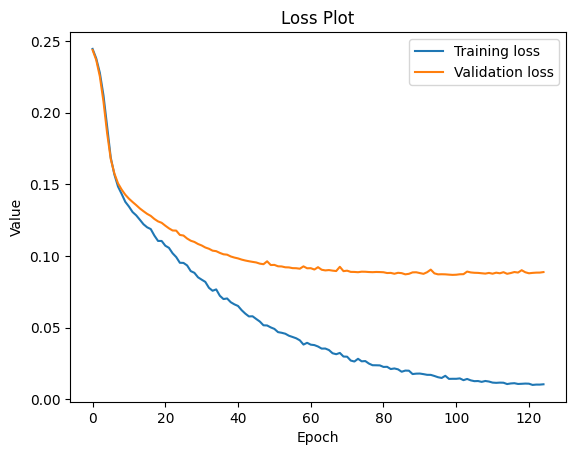
\includegraphics[scale=0.59]{assets/train_validation_loss.png}
  \caption{Train dan Validation Loss Curve}
  \label{fig:train_val_loss_cnn}
\end{figure}

\begin{figure}[H]
  \centering
  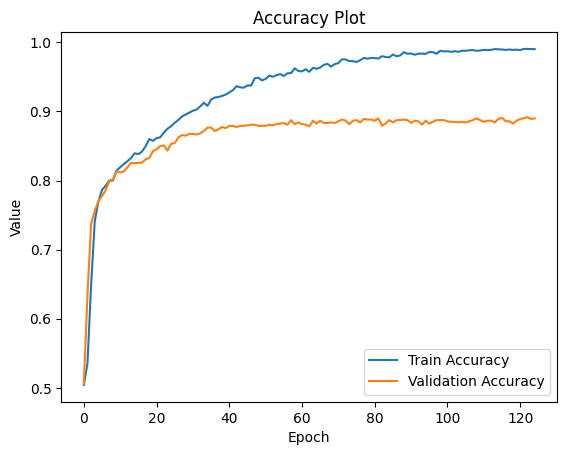
\includegraphics[scale=0.65]{assets/train_validation_accuracy.png}
  \caption{Train dan Validation Accuracy Curve}
  \label{fig:train_val_accuracy_cnn}
\end{figure}

Pelatihan model dilakukan dengan data latih dengan jumlah 3600 yang terdiri dari 1800 positif, dan 1800
negatif, data validasi dengan jumlah 1200 yang terdiri dari 600 positif dan 600 negatif, dan diuji menggunakan
data uji dengan jumlah 1200 yang terdiri dari 600 positif dan 600 negatif. Hasil proses dan kinerja dari
pelatihan model dapat dilihat pada Gambar~\ref{fig:train_val_accuracy_cnn} dan pada Gambar~\ref{fig:train_val_loss_cnn}.

\begin{figure}[H]
  \centering
  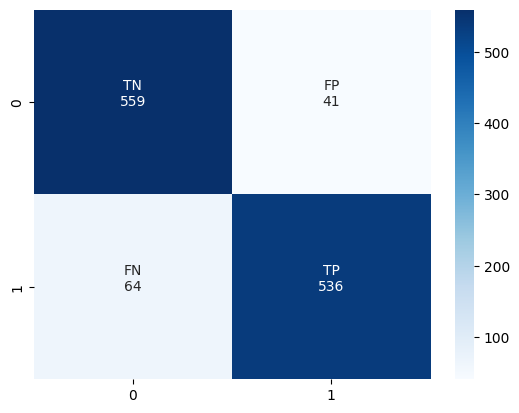
\includegraphics[scale=0.8]{assets/cm_heatmap.png}
  \caption{Confusion Matrix pada Data Uji}
  \label{fig:result_cm_testing}
\end{figure}

\begin{table}[H]
  \centering
  \caption{Laporan Hasil Klasifikasi}
  \label{tab:laporan_hasil_klasifikasi}
  \begin{tabular}{|lllll|}
    \hline
    \multicolumn{1}{|l|}{Label}             & \multicolumn{1}{l|}{\textit{Precision}} & \multicolumn{1}{l|}{\textit{Sensitivity}} & \multicolumn{1}{l|}{\textit{F-Measure}} & Jumlah \\ \hline
    \multicolumn{1}{|l|}{Positif}           & \multicolumn{1}{l|}{92,89\%}            & \multicolumn{1}{l|}{89,33\%}              & \multicolumn{1}{l|}{91,08\%}            & 600    \\ \hline
    \multicolumn{1}{|l|}{Negatif}           & \multicolumn{1}{l|}{89,73\%}            & \multicolumn{1}{l|}{93,17\%}              & \multicolumn{1}{l|}{91,41\%}            & 600    \\ \hline
    \multicolumn{5}{|l|}{}                                                                                                                                                           \\ \hline
    \multicolumn{1}{|l|}{Rata-Rata}         & \multicolumn{1}{l|}{91,31\%}            & \multicolumn{1}{l|}{91,25\%}              & \multicolumn{1}{l|}{91,25\%}            & 1200   \\ \hline
    \multicolumn{1}{|l|}{\textit{Accuracy}} & \multicolumn{3}{l|}{91,25\%}            & 1200                                                                                         \\ \hline
  \end{tabular}
\end{table}

Berdasarkan Tabel~\ref{tab:laporan_hasil_klasifikasi} dan Gambar~\ref{fig:result_cm_testing} kinerja
pada model yang dilakukan pengujian dengan data uji menghasilkan \emph{accuracy}, \emph{precision},
\emph{recall}, \emph{f1-score} dengan nilai berturut-turut 91,25\%, 91,31\%, 91,25\%, dan 91,25\%.
Contoh satu \emph{review} yang bernilai \emph{false positive} dan contoh satu \emph{review} bernilai \emph{false negative}
dapat dilihat pada Tabel~\ref{tab:sample_result_cm_testing}.

\begin{table}[H]
  \centering
  \caption{Sampel Data Uji yang Diklasifikasi}
  \label{tab:sample_result_cm_testing}
  \begin{tabularx}{\columnwidth}{|l|X|l|l|l|}
    \hline
    index & review                                                                                                                       & label   & prediksi & hasil          \\ \hline
    1     & Aplikasi kok gak jelas banget..ternyata masih nyaman di ijo aja lah..                                                        & negatif & positif  & False Positive \\ \hline
    2     & Langsung dapat orderan , tapi tidak ada driver yang datang ke resto , terus bagaimana ini, kasihan pelanggan nungguin. Sudah & positif & negatif  & False Negative \\ \hline
  \end{tabularx}
\end{table}
\newpage

Pada Tabel~\ref{tab:sample_result_cm_testing} dapat dilihat hasil dari klasifikasi terjadi karena kesalahan
model dalam memprediksi kalimat bersifat negatif atau positif. Untuk mengetahui penyebab dari kesalahan prediksi
dari model dapat dilakukan dengan cara melihat hasil praproses dan \emph{surrounding words} dari word2vec yang dapat dilihat
pada Tabel~\ref{tab:analysis_preprocess_predicted_test} dan Tabel~\ref{tab:analysis_mostsimilar_word2vec}.

\begin{table}[H]
  \centering
  \caption{Hasil Praproses Sampel Data Uji}
  \label{tab:analysis_preprocess_predicted_test}
  \begin{tabularx}{\columnwidth}{|l|X|X|}
    \hline
    index & review                                                                                                                       & preprocessed                                    \\ \hline
    1     & Aplikasi kok gak jelas banget..ternyata masih nyaman di ijo aja lah..                                                        & aplikasi tidak banget nyaman ijo                \\ \hline
    2     & Langsung dapat orderan , tapi tidak ada driver yang datang ke resto , terus bagaimana ini, kasihan pelanggan nungguin. Sudah & order tidak driver resto kasihan langgan tunggu \\ \hline
  \end{tabularx}
\end{table}

\begin{longtable}[c]{|l|l|l|l|}
  \caption{Surrounding Words Word2Vec}
  \label{tab:analysis_mostsimilar_word2vec}                                                                                                                                                              \\
  \hline
  preprocessed                                                                                                             & kata                         & serupa                   & nilai\_keserupaan \\ \hline
  \endhead
  \hline
  \endfoot
  %
  \multirow[t]{20}{*}{\begin{tabular}[t]{@{}l@{}}aplikasi\\ tidak\\ banget\\ nyaman\\ ijo\end{tabular}}                    & \multirow[t]{5}{*}{aplikasi} & browser                  & 72,91\%           \\ \cline{3-4}
                                                                                                                           &                              & plugin                   & 70,62\%           \\ \cline{3-4}
                                                                                                                           &                              & Aplikasi                 & 70,45\%           \\ \cline{3-4}
                                                                                                                           &                              & software                 & 69,59\%           \\ \cline{3-4}
                                                                                                                           &                              & server                   & 68,51\%           \\ \cline{2-4}
                                                                                                                           & \multirow[t]{5}{*}{banget}   & aja                      & 74,33\%           \\ \cline{3-4}
                                                                                                                           &                              & bikin                    & 73,77\%           \\ \cline{3-4}
                                                                                                                           &                              & nggak                    & 72,35\%           \\ \cline{3-4}
                                                                                                                           &                              & temen                    & 71,89\%           \\ \cline{3-4}
                                                                                                                           &                              & udah                     & 71,65\%           \\ \cline{2-4}
                                                                                                                           & \multirow[t]{5}{*}{nyaman}   & aman                     & 64,90\%           \\ \cline{3-4}
                                                                                                                           &                              & menyenangkan             & 62,45\%           \\ \cline{3-4}
                                                                                                                           &                              & betah                    & 61,68\%           \\ \cline{3-4}
                                                                                                                           &                              & kondusif                 & 60,52\%           \\ \cline{3-4}
                                                                                                                           &                              & santai                   & 60,46\%           \\ \cline{2-4}
                                                                                                                           & \multirow[t]{5}{*}{ijo}      & laos                     & 74,89\%           \\ \cline{3-4}
                                                                                                                           &                              & Jw                       & 74,42\%           \\ \cline{3-4}
                                                                                                                           &                              & jenang                   & 74,28\%           \\ \cline{3-4}
                                                                                                                           &                              & Lobak                    & 73,92\%           \\ \cline{3-4}
                                                                                                                           &                              & Buncis                   & 73,01\%           \\ \hline
  \multirow[t]{30}{*}{\begin{tabular}[t]{@{}l@{}}order\\ tidak\\ driver\\ resto\\ kasihan\\ langgan\\ tunggu\end{tabular}} & \multirow[t]{5}{*}{order}    & pre                      & 67,55\%           \\ \cline{3-4}
                                                                                                                           &                              & cost                     & 63,24\%           \\ \cline{3-4}
                                                                                                                           &                              & experience               & 61,95\%           \\ \cline{3-4}
                                                                                                                           &                              & challenge                & 61,68\%           \\ \cline{3-4}
                                                                                                                           &                              & job                      & 61,64\%           \\ \cline{2-4}
                                                                                                                           & \multirow[t]{5}{*}{tidak}    & tak                      & 79,03\%           \\ \cline{3-4}
                                                                                                                           &                              & belum                    & 66,92\%           \\ \cline{3-4}
                                                                                                                           &                              & tidaklah                 & 65,90\%           \\ \cline{3-4}
                                                                                                                           &                              & tanpa                    & 60,89\%           \\ \cline{3-4}
                                                                                                                           &                              & jika                     & 54,86\%           \\ \cline{2-4}
                                                                                                                           & \multirow[t]{5}{*}{driver}   & device                   & 66,25\%           \\ \cline{3-4}
                                                                                                                           &                              & client                   & 62,57\%           \\ \cline{3-4}
                                                                                                                           &                              & engine                   & 61,95\%           \\ \cline{3-4}
                                                                                                                           &                              & windows                  & 61,37\%           \\ \cline{3-4}
                                                                                                                           &                              & test                     & 61,12\%           \\ \cline{2-4}
                                                                                                                           & \multirow[t]{5}{*}{resto}    & restaurant               & 66,01\%           \\ \cline{3-4}
                                                                                                                           &                              & cafe                     & 65,77\%           \\ \cline{3-4}
                                                                                                                           &                              & caf\textbackslash{}u00e9 & 61,92\%           \\ \cline{3-4}
                                                                                                                           &                              & restoran                 & 60,86\%           \\ \cline{3-4}
                                                                                                                           &                              & kafe                     & 60,75\%           \\ \cline{2-4}
                                                                                                                           & \multirow[t]{5}{*}{kasihan}  & kasihannya               & 76,93\%           \\ \cline{3-4}
                                                                                                                           &                              & kasihnya                 & 73,59\%           \\ \cline{3-4}
                                                                                                                           &                              & kasih                    & 61,90\%           \\ \cline{3-4}
                                                                                                                           &                              & dengki                   & 56,38\%           \\ \cline{3-4}
                                                                                                                           &                              & penyesalan               & 56,34\%           \\ \cline{2-4}
                                                                                                                           & \multirow[t]{5}{*}{tunggu}   & ditunggu                 & 58,61\%           \\ \cline{3-4}
                                                                                                                           &                              & PPKA                     & 56,31\%           \\ \cline{3-4}
                                                                                                                           &                              & tunggunya                & 50,91\%           \\ \cline{3-4}
                                                                                                                           &                              & Tunggu                   & 49,32\%           \\ \cline{3-4}
                                                                                                                           &                              & keberangkatan            & 49,23\%           \\ \hline
\end{longtable}

Berdasarkan Tabel~\ref{tab:analysis_preprocess_predicted_test} dan Tabel~\ref{tab:analysis_mostsimilar_word2vec}
pada index ke-1 hasil praproses terdapat kata `banget' dan `nyaman' yang memiliki \emph{surrounding word}
yang memiliki makna positif maka model memprediksi kalimat memiliki label positif, sedangkan untuk
di index ke-2 terdapat kata `tidak', `kasihan', dan `tunggu' yang memiliki \emph{surrounding words}
yang memiliki makna negatif maka model memprediksi kalimat memiliki label negatif.


\section{Kesimpulan}
Kesimpulan dari pengujian model pada data uji yang telah dilakukan adalah parameter yang menghasilkan
kinerja model terbaik terdapat pada skenario 20 dengan nilai parameter epoch = 125, batch\_size = 8 dan
word2vec\_trainable = false, activation = sigmoid, optimizer = adam, learning\_rate = 0.00001,
convolution\_activation = relu, dan loss = mse yang menghasilkan nilai \emph{accuracy},
\emph{precision}, \emph{recall}, dan \emph{f1-score} berturut-turut 91,25\%, 91,31\%, 91,25\%, dan 91,25\%.